\documentclass[tikz,border=10pt]{standalone}
\usepackage{tikz}
\usetikzlibrary{positioning}
\usepackage{tikz-feynman} % texdoc tikz-feynman 
\begin{document}

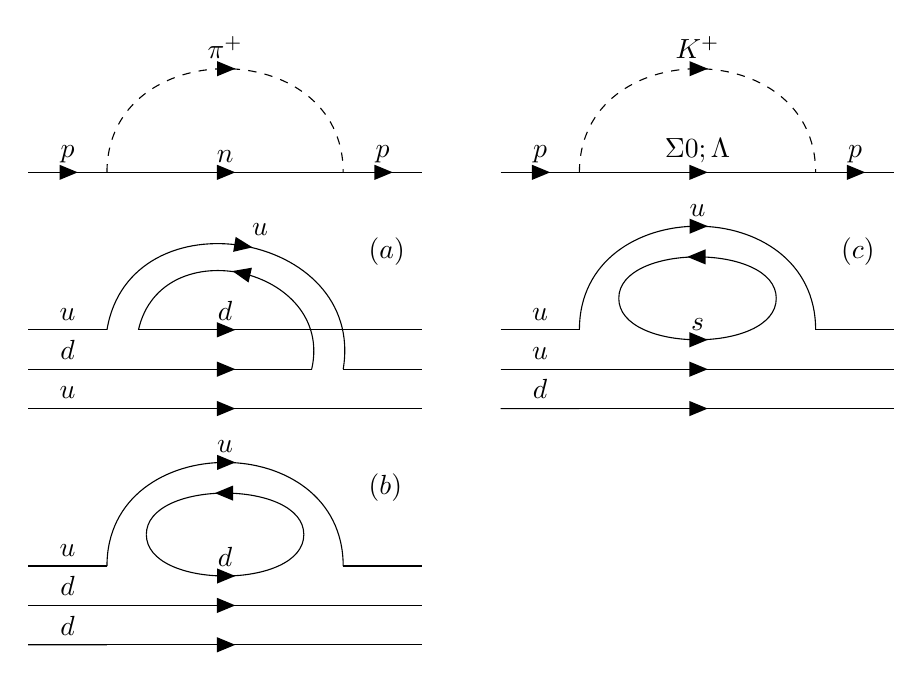
\begin{tikzpicture}
	\begin{feynman}
		%% 图 x
		\vertex (x1) at (0,0);
		\vertex[right =1cm  of x1] (x2);
		\vertex[right =2.5cm  of x1] (x3);
		\vertex[right =4cm  of x1] (x4);
		\vertex[right =5cm  of x1] (x5);
		%% 图 y
		\vertex[right =6 of x1] (y1);
		\vertex[right =1cm  of y1] (y2);
		\vertex[right =2.5cm  of y1] (y3);
		\vertex[right =4cm  of y1] (y4);
		\vertex[right =5cm  of y1] (y5);
		%% 子图 a
		\vertex[above =-2 of x1] (a1);
		\vertex[right =1  of a1] (a2);
		\vertex[above =-0.5  of a2] (a2d);
		\vertex[above =-0.5  of a2d] (a2dd);
		\vertex[right =1.4  of a1] (a3);
		\vertex[above =-0.5  of a3] (a3d);
		\vertex[right =3.6  of a1] (a4);
		\vertex[right =4  of a1] (a5);
		\vertex[right =5  of a1] (a6);
		\vertex[above =-0.5 of a1] (a7);
		\vertex[right =3.6 of a7] (a8);
		\vertex[right =4 of a7] (a9);
		\vertex[right =5 of a7] (a10);
		\vertex[above =-0.5 of a7] (a11);
		\vertex[right =5 of a11] (a12);
		\node[above right =0.7 and 4.2 of a1] {$(a)$};
		%% 子图 b
		\vertex[above =-5 of x1] (b1);
		\vertex[right =1  of b1] (b2);
		\vertex[above =-0.5  of b2] (b2d);
		\vertex[above =-0.5  of b2d] (b2dd);
		\vertex[right =4  of b1] (b3);
		\vertex[right =5  of b1] (b4);
		\vertex[above =-0.5 of b1] (b5);
		\vertex[right =5  of b5] (b6);
		\vertex[above =-1 of b1] (b7);
		\vertex[right =5  of b7] (b8);
		\vertex[above right =0.4 and 1.5  of b1] (b9);
		\vertex[above right =0.4 and 3.5  of b1] (b10);
		\node[above right =0.7 and 4.2 of b1] {$(b)$};
		%% 子图 c
		\vertex[above =-2 of y1] (c1);
		\vertex[right =1  of c1] (c2);
		\vertex[above =-0.5  of c2] (c2d);
		\vertex[above =-0.5  of c2d] (c2dd);
		\vertex[right =4  of c1] (c3);
		\vertex[right =5  of c1] (c4);
		\vertex[above =-0.5 of c1] (c5);
		\vertex[right =5  of c5] (c6);
		\vertex[above =-1 of c1] (c7);
		\vertex[right =5  of c7] (c8);
		\vertex[above right =0.4 and 1.5  of c1] (c9);
		\vertex[above right =0.4 and 3.5  of c1] (c10);
		\node[above right =0.7 and 4.2 of c1] {$(c)$};
		% 对各个顶点连线
		\diagram*{
		%普通连线
		{ [edge= plain]
		(a1) --[edge label =\(u\)] (a2),(a9)--(a10),(a4)--(a6),
		(a7) --[edge label =\(d\)] (a2d)--(a3d),(a9) -- (a10),
		(a11)--[edge label =\(u\)](a2dd),
		%%%
		(b3)--(b4),
		(b1)--[edge label =\(u\)](b2),
		(b5)--[edge label =\(d\)](b2d),
		(b7)--[edge label =\(d\)](b2dd),
		%%%
		(c3)--(c4),
		(c1)--[edge label =\(u\)](c2),
		(c5)--[edge label =\(u\)](c2d),
		(c7)--[edge label =\(d\)](c2dd),
		},
		%费米子箭头连线
		{ [edge= fermion]
		(x1) --[edge label =\(p\)](x2)--[edge label =\(n\)](x4) --[edge label =\(p\)](x5),
		%%%
		(a3) --[edge label =\(d\)] (a4),(a3d)--(a8),(a11)--(a12),
		(a2) --[half left,looseness=1.5,edge label =\(u\)](a9),(a8) --[half right,looseness=1.5](a3),
		%%%
		(b5)--(b6),(b7)--(b8),
		(b2) --[half left,looseness=1.5,edge label =\(u\)](b3),
		(b9) --[half right,looseness=0.9,edge label =\(d\)](b10) --[half right,looseness=0.9](b9),
		%%%
		(y1) --[edge label =\(p\)](y2)--[edge label =\(\Sigma0;\Lambda\)](y4) --[edge label =\(p\)](y5),
		%%%
		(c5)--(c6),(c7)--(c8),
		(c2) --[half left,looseness=1.5,edge label =\(u\)](c3),
		(c9) --[half right,looseness=0.9,edge label =\(s\)](c10) --[half right,looseness=0.9](c9),
		},
		% 介子连线
		{ [edge= charged scalar]
		(x2) --[half left,edge label =\(\pi^{+}\)](x4),
		(y2) --[half left,edge label =\(K^{+}\)](y4),
		}
		};
	\end{feynman}
\end{tikzpicture}

\end{document}
